\documentclass[12pt]{article}

% Basics
\usepackage{sbc-template}
\usepackage{graphicx,url}
\usepackage[brazil]{babel}
\usepackage[utf8]{inputenc}
\usepackage{csquotes}           % ensuring that PT-BR quoting rules are used
\usepackage{amsmath}

% Figures
\usepackage{graphicx}
\graphicspath{ {images/} }
\usepackage{caption}
\usepackage{subfig}

% allows using [H] option on figure
\usepackage{float}

% Referencing
\usepackage{biblatex}
\addbibresource{references.bib}

% Using algorithms
\usepackage{xcolor}
\usepackage[nice]{nicefrac}
\usepackage{listings}
\usepackage[options]{algorithm2e}

% Setting page numbers
\pagestyle{plain}
\pagenumbering{arabic}

% Configurando as listagens (ver https://en.wikibooks.org/wiki/LaTeX/Source_Code_Listings)
\renewcommand{\lstlistingname}{Algoritmo}
\lstset{language=C, %C, mas a sintaxe é pseudo-Pascal
              belowcaptionskip=1\baselineskip,
                breaklines=true,
                frame=single,
                xleftmargin=\parindent,
                showstringspaces=false,
                basicstyle=\footnotesize\ttfamily,
                keywordstyle=\bfseries,
                commentstyle=\itshape,
                stringstyle=\color{orange},
                numbers=left,
                rulecolor=\color{black},
                aboveskip=2em,
                belowskip=-2em,
                morekeywords={procedure, then, to},
                backgroundcolor=\color{gray!10},
                extendedchars=false,
                inputencoding=utf8,
            }


\sloppy

\title{Comparação entre resultados teóricos e práticos do tempo de execução em algoritmos de ordenação}

\author{Luiz C. F. Ribeiro}

\address{Pós-Graduação em Ciência da Computação -- Universidade Estadual Paulista (UNESP)
  \email{lzcfelix@gmail.com}
}

\begin{document} 

\maketitle

\begin{resumo}
Este trabalho descreve a complexidade teórica dos algoritmos de ordenação mais comuns e as relaciona com resultados experimentais. Os resultados obtidos para cada tipo de análise são complementares, de forma que \textit{Quick} e \textit{Merge sort} consistem, de maneira geral, em boas escolhas quando deseja-se minimzar o tempo gasto nesta operação.
\end{resumo}


\section{Introdução}

A análise da complexidade assintótica de um algoritmo consiste na utilização de técnicas matemáticas que permitem prever a quantidade de recursos, seja em termos de tempo ou memória (espaço), que este irá consumir para todas suas possíveis entradas, sem que haja a necessidade de implementá-lo. Apesar disso, esta abordagem ignora diversos fatores que surgem na prática, por exemplo, instruções que não sejam atribuição e comparação possuem custo de execução zero, aspectos de \textit{hardware} como \textit{cache miss} e de \textit{software}, como a sobrecarga causada pela interpretação do programa, também não são considerados.

Em contrapartida, a análise puramente experimental torna difícil a comparação entre resultados obtidos em diferentes configurações, já que tais análises são fortemente dependentes do \textit{hardware} utilizado, da linguagem de programação escolhida, além do ambiente de testes estar sujeito a fatores que não podem ser controlados, como é o caso de processos executados em segundo plano pelo sistema operacional. Tais fatores dificultam a reproducibilidade dos experimentos realizados.

Uma forma de realizar análises mais compreensivas dos algoritmos, especialmente em termos de tempo de execução, consiste em comparar os resultados assintóticos com aqueles obtidos experimentalmente, permitindo que as características positivas dos dois tipos de análises sejam combinadas.

O foco deste trabalho consiste em analisar a complexidade de diferentes algoritmos de ordenação, já que existe ampla literatura sobre o assunto e sua implementação não é tão complexa. Os algoritmos aqui apresentados foram implementados utilizando a linguagem Python 3.5\footnote{www.python.org/downloads/release/python-350/} e a medição dos tempos de execução foi realizada por meio da biblioteca \texttt{timeit}\footnote{docs.python.org/3/library/timeit}, disponibilizada nativamente pela linguagem.

Cada algoritmo de ordenação foi executado dez vezes para cada conjunto de dados para o cálculo do tempo médio de execução e seu desvio padrão. Os experimentos foram executados em um computador com processador Intel Dual Core E2200 2.20GHz, com 2GB de memória RAM e sistema operacional Debian 8.

Os conjuntos de dados utilizados para testes consistem em arranjos com números inteiros em ordem crescente, decrescente e não ordenados (ou embaralhados). Nos dois primeiros casos, as entradas contém os números no intervalo $[0,n)$, onde $n$ é o tamanho do arranjo. No último caso os \textit{arrays} possuem valores distribuídos uniformemente entre $[0,k]$, com $k=2^{16} - 1$.

Para os algoritmos de complexidade quadrática, foram utilizados conjuntos de entradas com 1000, 5000, 10000, 15000, 20000, 25000 e 30000 elementos. Entradas maiores passam a demandar quantidade consideravel de tempo para a execução dos testes em todos cenários. 

Para os demais algoritmos, além destas entradas, conjuntos com 50, 100, 200, 300, 400 e 500 mil elementos também foram utilizados, possibilitando a visualização de tendências de uma forma mais geral, conforme pode ser observado nos gráficos de desempenho.





\section{\textit{Bubble sort}}

Este algoritmo, assim como os demais métodos de complexidade quadrática, possui dois laços de repetição aninhados: $I$, com contador $i$ e $J$, com contador $j$, sendo o primeiro \textit{loop} externo e o segundo interno.

$J$ itera o array comparando o valor da posição $j$ com seu sucessor e troca estes elementos de lugar se $v[j] > v[j+1]$. Isso faz com que ao fim de cada iteração de $J$, o $i$-ésimo maior elemento do conjunto de entrada esteja em sua posição final (ou ordenada) no array. Consequentemente, na iteração seguinte $J$ deve percorrer o arranjo até a posição $(n-i)$. Quando $I$ termina todas suas iterações, $i=n$ e pela propriedade anterior, o \textit{array} está ordenado.

O funcionamento do algoritmo pode ser descrito por meio da Equação \ref{eq:soma_quadratica}, mostrando que este é, de fato, de ordem quadrática.

\begin{equation}
\label{eq:soma_quadratica}
\begin{aligned}
    T(n) = &\; (n-1)+(n-2)+\underbrace{\ldots}_{\substack{\text{(n-5)} \\ \text{termos}}}+2+1 \\
         = & \sum_{t=1}^{n-1}t = \frac{n(n+1)}{2} - n = n^2-n  \in \mathcal{O}(n^2)
\end{aligned}
\end{equation}

Como o conjunto de entrada é considerado ordenado apenas ao fim das iterações de $I$ e o loop $J$ é linear, o comportamento do algoritmo independe do conjunto de entrada, fator que permite restringir sua complexidade para $\Theta(n^2)$.

Ao analisar os resultados experimentais exibidos na Figura \ref{fig:bubble_sort}, é possível concluir que o tempo de execução do algoritmo é maior em conjuntos de dados em ordem decrescente (pior caso) que crescente (melhor caso).

Isso se deve ao fato de que no pior caso cada elemento do arranjo, além de ser comparado com todos seus $n-i$ sucessores, também é trocado com todos os demais, fazendo com que $U(n) = 2(n^2-n)$ operações sejam realizadas. Ainda assim, $U(n) \in \mathcal{O}(n^2)$, apesar da constante oculta pela notação assintótica influenciar consideravelmente o tempo de execução do algoritmo.

Já no melhor caso, o algoritmo apenas realiza a comparação entre elementos, sem efetuar trocas, tendo em vista que o conjunto de entrada já encontra-se ordenado.

Por fim, o arranjo embaralhado consiste no caso médio, pois a deslocação de elementos, responsável pelo trabalho adicional no pior caso, ocorre com menor frequência, devido a distribuição aleatória dos valores no arranjo.

\begin{figure}[h]%    
    \subfloat{{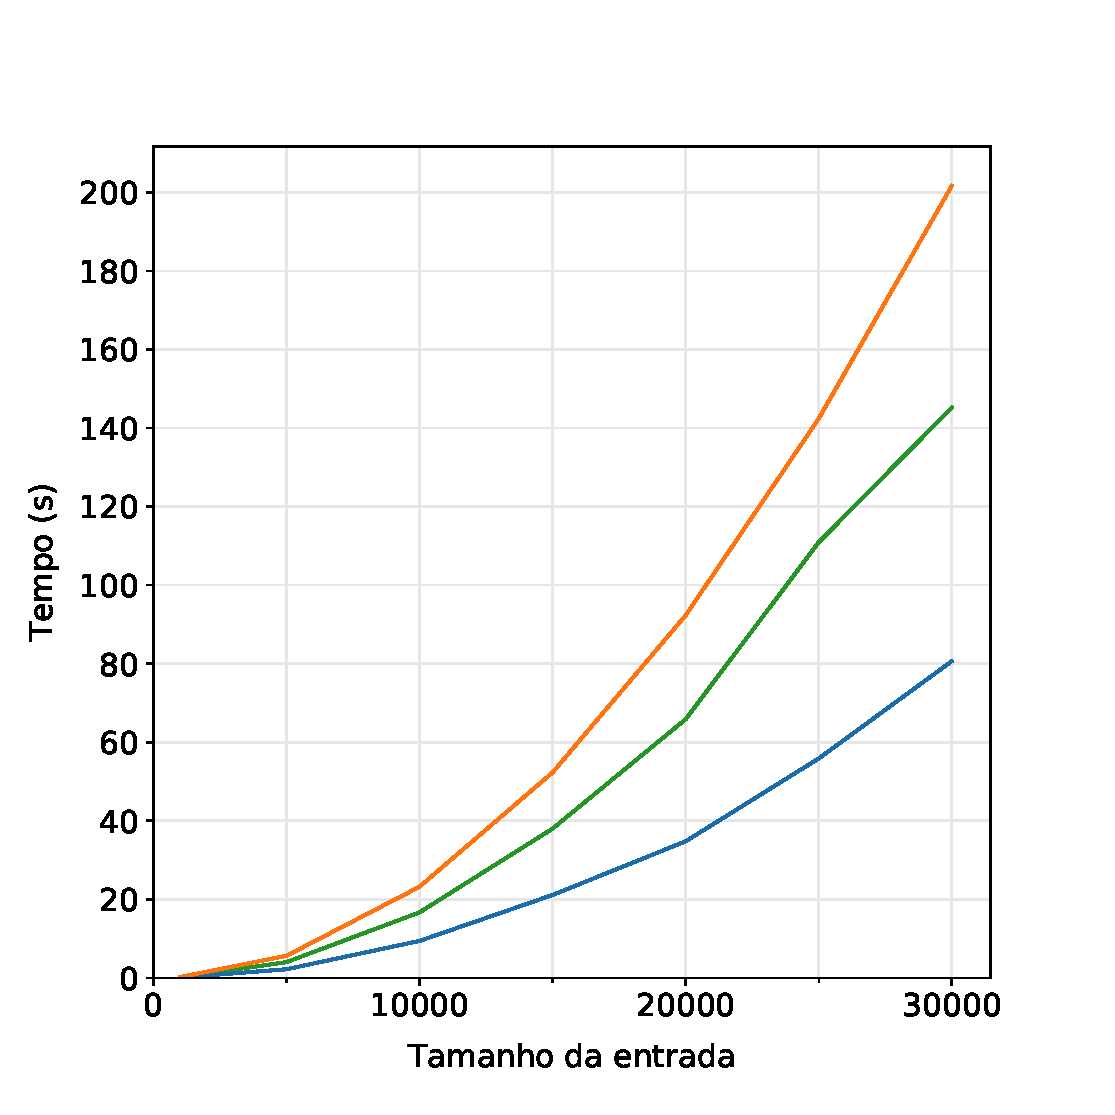
\includegraphics[width=0.5\textwidth]{bubble} } \label{fig:bubble_sort}}%
    \subfloat{{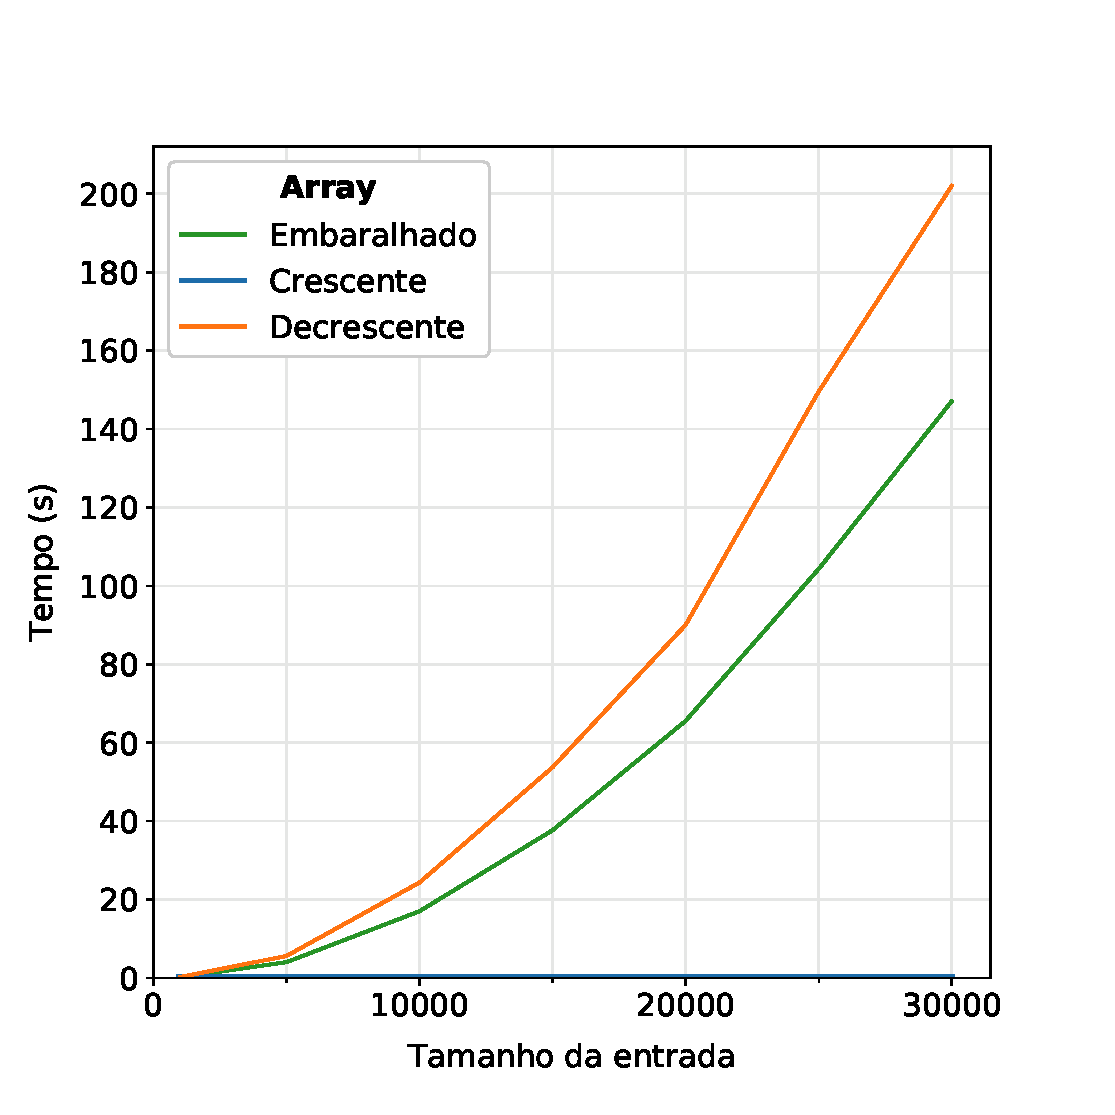
\includegraphics[width=0.5\textwidth]{bubble_improved} } \label{fig:bubble_sort*}}%
    \caption{Resultados experimentais para as implementações normal (a) e melhorada (b) do \textit{Bubble sort}}%
    \label{fig:bubble}%
\end{figure}

\section{\textit{Bubble sort} melhorado}

A implementação original do \textit{Bubble sort} é incapaz de identificar situações onde o conjunto de entrada já está ordenado ou quando o arranjo fica ordenado antes do loop $I$ terminar. Além disso, apesar da análise assintótica determinar que o algoritmo possui a mesma complexidade para todos os casos, o experimento anterior mostra que o algoritmo executa consideravelmente mais rápido quando o \textit{array} já está ordenado, consistindo no melhor caso prático.

Assim, é interessante alterar o funcionamento deste método a fim de melhorar seu desempenho neste cenário, já que este comportamento impacta sua complexidade no melhor caso, e consequentemente, seu limitante inferior.

Suponha que após $k$ iterações de $I$, com $k<n$, o arranjo esteja ordenado, ou seja, $v[t] < v[t+1]$ para todo o \texit{array}. Nas próxima iteração de $J$, a expressão de troca de elementos $v[j] > v[j+1]$ sempre será falsa. Consequentemente pode-se concluir que o conjunto de entrada encontra-se ordenado e o algoritmo pode então terminar antecipadamente.

Essa mudança faz com que o Bubble Sort seja $\Omega(n)$ para entradas ordenadas, já que o \textit{loop} $J$ deve ser executado ao menos uma vez a fim de verificar se a condição anteior é sempre falsa. Além disso, o número de operações realizadas para entradas parcialmente ordenadas também diminui. Apesar dessas mudanças, o método continua sendo $\mathcal{O}(n^2)$ no pior caso.

Os resultados da análise experimental são mostrados na Figura \ref{fig:bubble_sort*}, corroborando com o argumento de que as modificações alteram a complexidade do método apenas no melhor caso. Note que apesar do algoritmo ser $\Omega(n)$, o tempo de execução no gráfico é descrito por uma reta aproximadamente constante e próxima a zero e não próxima à abcissa dos quadrantes ímpares.

Esse aspecto se deve aos seguintes fatores: o gráfico é função do tempo de execução, e não quantidade de instruções, pelo tamanho da entrada; a eficiência em realizar acessos estritamente sequenciais à memória aumenta o aproveitamento das memórias de cache pelo algoritmo. Por fim, o fato dos dados estarem ordenados provavelmente faz com que o \textit{branch prediction} realizado pelo processador também interfira positivamente no tempo de execução do algoritmo, já que a comparação efetuada em $J$ é sempre falsa.



\section{\textit{Selection sort}}

Neste algoritmo, o menor elemento do \textit{array} é procurado e inserido em sua primeira posição. A seguir, o próximo menor elemento é encontrado e movido para sua segunda posição e assim sucessivamente até que todo o arranjo esteja ordenado.

Deste modo, ao final de cada iteração de $I$, os $i$ menores elementos do conjunto de entrada estão em suas posições ordenadas. Para isso, a cada execução do laço externo, $J$ busca o menor valor no sub-array $v[i..n]$ e troca este elemento de lugar com $v[i]$.

Esse procedimento também faz com que gradativamente sejam formadas duas partições no \textit{array}, $v[1..i]$ e $v[i+1..n]$. Enquanto a partição direita contém elementos potencialmente embaralhados, a esquerda possui seus elementos ordenados, sendo que a cada iteração esta é acrescida de um novo elemento, removido da outra partição.% Este procedimento é similar ao particionamento realizado pelo Insertion Sort.

Como $J$ percorre apenas os elementos da segunda partição do arranjo, este deve percorrer apenas os $n-i$ números no sub-array $v[i..n]$ em busca do menor valor, procedimento que se repete $n$ vezes. Logo, o algoritmo pode ser descrito pela Equação \ref{eq:soma_quadrativa_inversa}, que equivale a (\ref{eq:soma_quadratica}).

\begin{equation}
\label{eq:soma_quadrativa_inversa}
\begin{aligned}
    T(n) = n + (n-1) + \ldots + 1 = n^2-n \in \mathcal{O}(n^2)
\end{aligned}
\end{equation}

Assim como no \textit{Bubble sort}, o \textit{array} é considerado ordenado apenas quando a execução de $I$ chega ao fim, já que não é realizada nenhuma verificação intermediária a respeito da disposição dos elementos no arranjo. Isso faz com que a complexidade do algoritmo seja indiferente a organização do conjunto de entrada. Isso faz com que, novamente, $\mathcal{O}(n^2)$ pode ser restrito a $\Theta(n^2)$.

Os resultados experimentais são exibidos na Figura \ref{fig:selection}, onde é possível perceber que os tempos de execução do algoritmo são consideravelmente menores quando comparados à implementações do \textit{Bubble sort}, a menos das entradas ordenadas em sua segunda versão.

A rapidez de execução do \textit{Selection sort} se deve ao fato de que a cada iteração apenas dois elementos do conjunto de entrada são permutados, diminuindo a quantidade de operações de escrita realizadas no mesmo. Essa característica também faz com que seu custo, em termos de tempo computacional seja bastante próximo em todos os casos..

Para justificar as pequenas variações de tempo entre os casos de execução, considere o Algoritmo \ref{alg:selection_sort}. No melhor caso (arranjo ordenado), o primeiro valor da partição direita sempre será o menor elemento, ou seja, aquele que deve ser inserido na região ordenada. Isso faz com que apenas as comparações em $J$ sejam realizadas.

Por outro lado, para o pior caso (array em ordem decrescente), a cada iteração de $J$ além da comparação, a etapa de armazenamento do menor valor parcial (linhas 8 e 9 do algoritmo) sempre será executada. Isso faz com que o tempo de execução do Selection Sort aumente ligeiramente.

Por fim, para o caso médio (vetor embaralhado) a posição do menor elemento na partição direita é aleatória, logo a atribuição realizada na linha 9 será executada $k$ vezes. Se $k=n$ então trata-se do pior caso, mas se $k=0$, o conjunto de entrada já está ordenado e este é o melhor caso.

\begin{lstlisting}[caption=Selection Sort, float, label=alg:selection_sort, captionpos=b, h]
procedure selectionSort(v, n)
    for i := 1 to n do               /*loop I*/
        jmin := i
        val_min := v[i]
        
        /* busca pelo i - ésimo menor elemento*/
        for j := i+1 to n do        /* loop J */
            if (val_min > v[j]) then
                jmin := j
                val_min := v[j]
        
        swap(v[i], v[jmin])
\end{lstlisting}




\section{\textit{Insertion sort}}

Este algoritmo também se baseia na divisão do conjunto de entrada em duas partições. Enquanto a esquerda contém os elementos ordenados e inicialmente está vazia, a segunda está potencialmente fora de ordem e representa todo o arranjo.

A cada iteração de $I$, o primeiro elemento $p$ da partição direita é removido e o algoritmo procura a posição ideal para inserí-lo na região esquerda, de forma que esta continue ordenada. Nesta etapa, o loop $J$ percorre todas posições da primeira região, que contém $i$ elementos, da direita para esquerda (ou do fim para o começo) até que um elemento $v[j] < p$ seja encontrado. Quando isso acontece, $p$ é inserido na posição $j+1$. Ao realizar esse procedimento, a região esquerda é acrescida de um elemento, enquanto a direita perde uma posição. O Algoritmo \ref{alg:insertion_sort} ilustra o funcionamento do \textit{Insertion sort}.

\begin{lstlisting}[caption=Insertion Sort, float, label=alg:insertion_sort, captionpos=b, h]
procedure insertionSort(v, n)
    for i := 2 to n do                       /*loop I*/
        p := v[i]
        while (j >= 2 and v[j-1] > p) do    /* loop J*/
            /*movimentacao dos elementos da particao esquerda*/
            v[j] := v[j+1]
            j := j-1
        /*insercao na posicao ideal*/
        v[j] := p
\end{lstlisting}

Note que a inserção de $p$ na posição $j+1$ exige que todos elementos no \textit{array} entre $j+1$ e $i$ sejam movidos uma posição adiante, procedimento que possui complexidade linear. Apesar dessa tarefa ser realizada junto com a busca pela posição ideal de inserção, cada novo elemento adicionado à partição esquerda incorre o custo de $(j-i+1)$ operações de escrita no arranjo.

Para determinar o pior caso de execução do algoritmo, suponha que o conjunto de entrada esteja em ordem decrescente. Neste caso, $p$ será sempre menor que todos elementos na partição ordenada, fazendo com que $i-1$ comparações sejam realizadas a cada iteração, a fim de determinar a posição ideal de inserção, que será sempre $v[0]$.

Inicialmente a primeira região estará vazia, logo nenhuma comparação é realizada. Na segunda iteração, uma comparação é realizada, a seguir, três, e assim sucessivamente, conforme descrito na Equação \ref{eq:soma_quadratica_progressiva}, que equivale a Equação \ref{eq:soma_quadratica}. Portanto para esta situação o \textit{Insertion Sort} é $\mathcal{O}(n^2)$, onde o custo da movimentação nos elementos do \textit{array} é oculto pela notação \cite{algorithms_redbook}.

\begin{equation}
\label{eq:soma_quadratica_progressiva}
    T(n) = 0+1+\underbrace{\ldots}_{\substack{\text{(n-5)} \\ \text{termos}}}+(n-2)+(n-1) = \sum_{t=0}^{n-1}t \in \mathcal{O}(n^2)
\end{equation}

Quando o conjunto de entrada possui todos seus elementos em ordem crescente, $p$ sempre será maior que todos os elementos na partição esquerda. Isso faz com que a comparação entre elemetos ocorre uma vez a cada iteração de $I$, já que $v[i] < p$ e $v[i+1] = p$. Como esta situação ocorre $n$ vezes, o algoritmo executa $\Omega(n)$ operações, consistindo no melhor caso.

Finalmente, o arranjo embaralhado consiste no caso médio. Se este possuir elementos distribuídos de maneira completamente aleatória, de acordo com a análise anterior, o algoritmo apresentará comportamento quadrático. Entretanto, caso o conjunto de entrada esteja parcialmente ordenado, o algoritmo explorará essas regiões exibindo comportamento linear, consequentemente diminuindo o tempo necessário para a ordenação. É seguro então dizer que o algoritmo realiza, no máximo, $\mathcal{O}(n^2)$ operações nesta situação.

A Figura \ref{fig:insertion} mostra os resultados obtidos empiricamente. O tempo de execução para entradas ordenadas é constante e próximo a zero, levando em consideração as mesmas observações realizadas na discussão sobre a melhoria do algoritmo \textit{Bubble sort}.

O \textit{array} embaralhado consiste no caso médio, descrevendo uma parábola para seu tempo de execução, enquanto o pior caso descreve o mesmo comportamento, mas com crescimento mais acentuado, atestando a análise teórica realizada.

Apesar de ser extremamente rápido para entradas ordenadas (e parcialmente ordenadas), nos demais casos este algoritmo é mais lento que o \textit{Selection sort}.


\begin{figure}[!h]%    
    \subfloat{{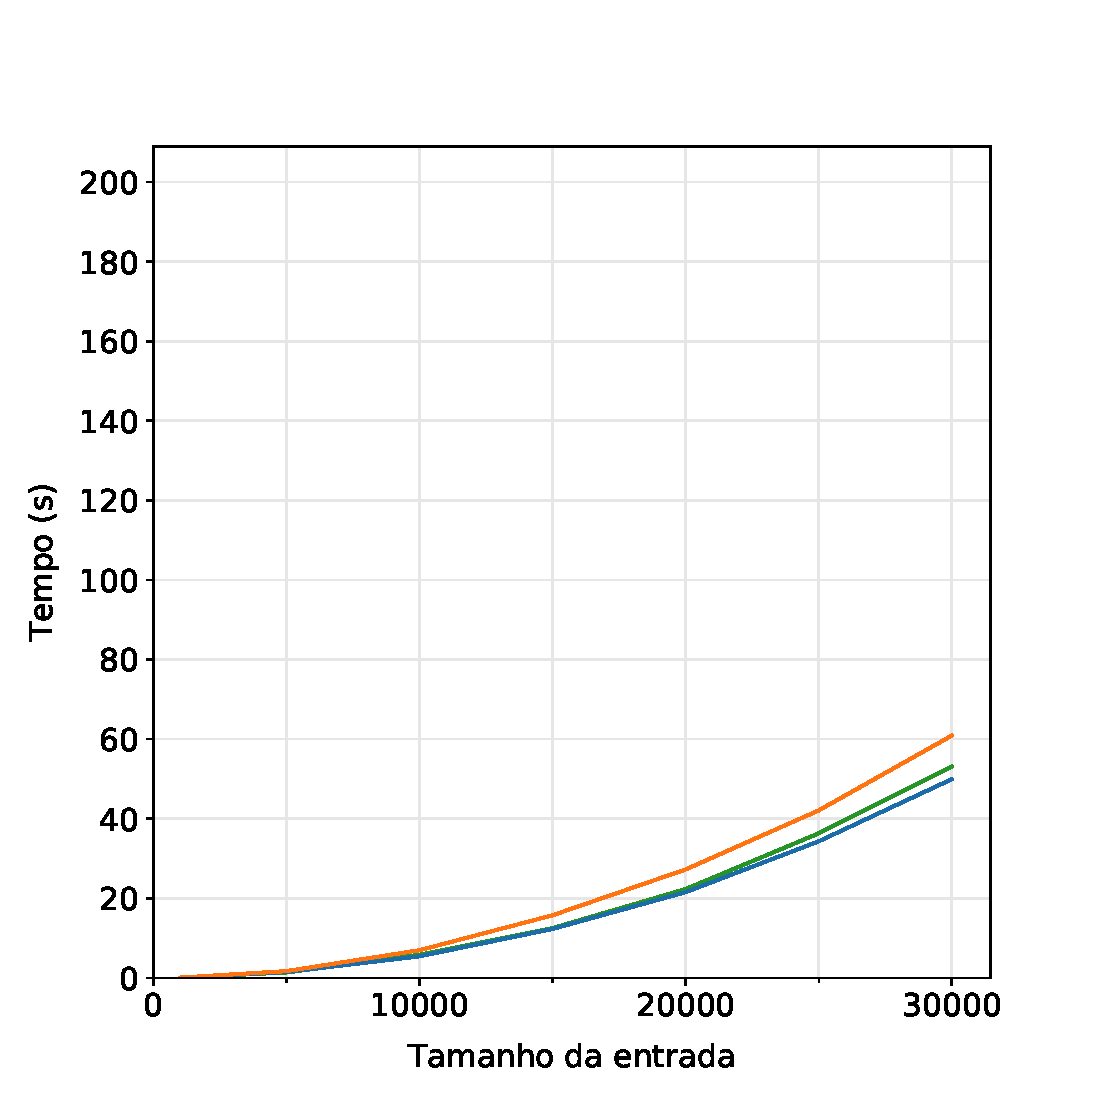
\includegraphics[width=0.5\textwidth]{selection} } \label{fig:selection}}%
    \subfloat{{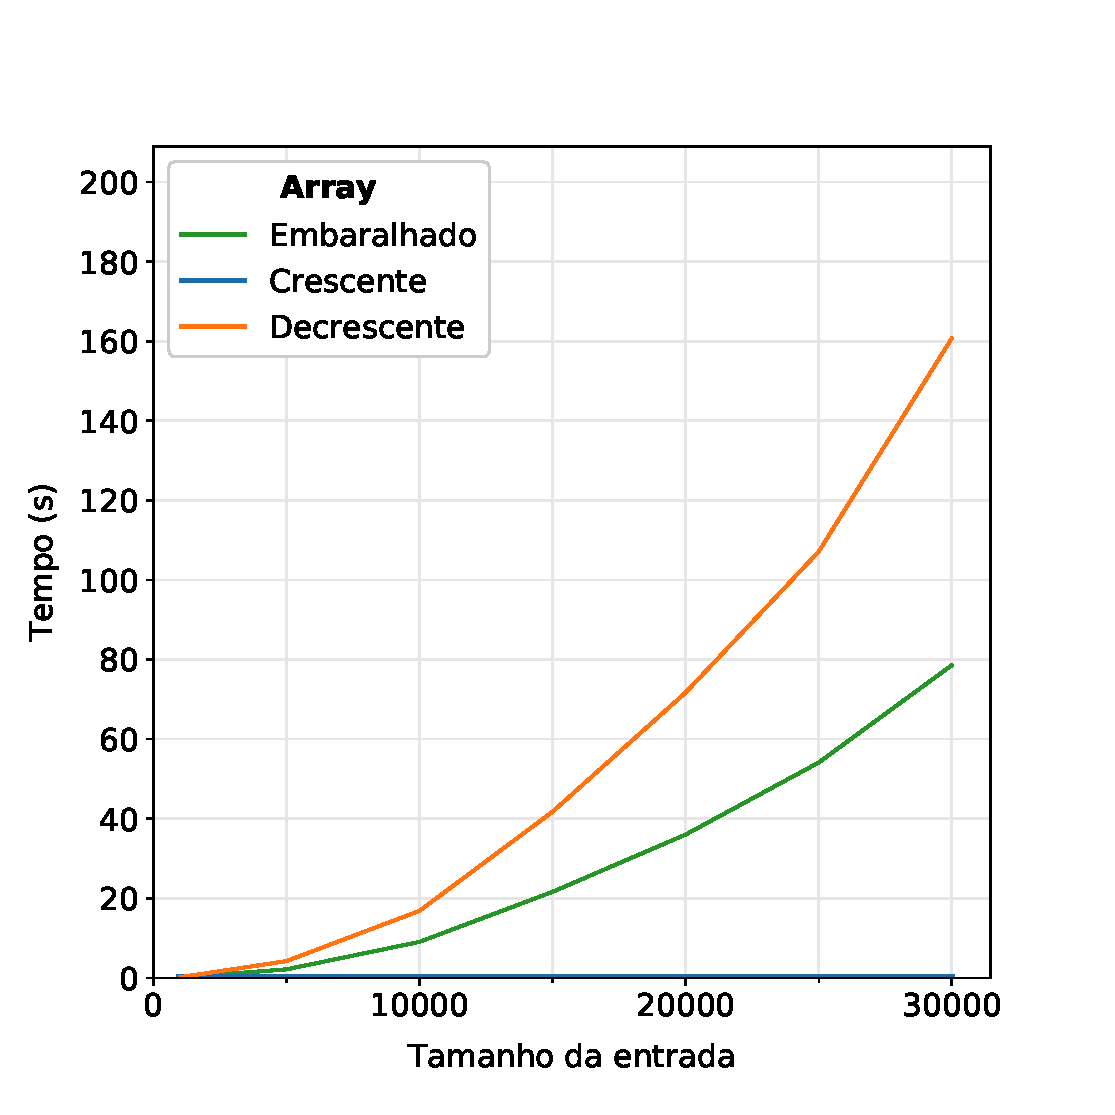
\includegraphics[width=0.5\textwidth]{insertion} } \label{fig:insertion}}%
    \caption{Tempos de execução experimentais para o \textit{Selection} (a) e \textit{Insertion sort} (b)}%
\end{figure}





\section{\textit{Shell Sort}}

A ideia deste algoritmo consiste em explorar a o fato de que o \textit{Insertion sort} apresenta comportamento próximo ao linear para ordenar arranjos parcialmente ordenados. A fim de se beneficiar desse fato, o \textit{Shell sort} divide o conjunto de entrada em várias partições, que são ordenadas paralelamente utilizando a ordenação por inserção. A seguir, estas partições são gradativamente combinadas, gerando um arranjo quase-ordenado, que então é submetido ao \textit{Insertion sort}, onde novamente espera-se que o algoritmo apresente um bom desempenho.

Uma sequência é utilizada na determinação do tamanho dos saltos a cada iteração para formar os sub-arranjos. Considere, por exemplo, $s = \{4, 2, 1\} = \{2^i\}$. Na iteração inicial, cada partição conterá os elementos respectivamente nas posições $v[4t], v[4t+1], v[4t+2], v[4t+3]$. 
Os sub-arranjos são então ordenados atrabés do \textit{Insertion sort} e então novas partições são formadas utilizando saltos agora de tamanho 2. Isso faz com que desta vez existam dois arranjos, um com os elementos nas posições $v[2t]$ e outro com os valores das posições $v[2t+1]$. Ao fim desta etapa de ordenação, o novo tamanho de salto é 1, de modo que todo o \textit{array}, que já encontra-se parcialmente ordenado é processado em sua totalidade.

A determinação da complexidade do \textit{Shell sort} depende diretamente da sequência de saltos utilizada, sendo este um problema ainda aberto. Knuth \cite{art_cc3} trata as possibilidades de escolha de maneira bem completa, relacionando este problema a outras áreas da Matemática.

Sabe-se que a sequência utilizada anteriormente faz com que o algoritmo apresente complexidade quadrática, entretanto a utilização da sequência $h = \{2^i-1\}$ torna o mesmo algoritmo $\mathcal{O}(n^{\nicefrac{3}{2}})$ \cite{hibbard_sequence}. Na implementação para realização dos experimentos esta última opção foi utilizada. Várias outras sequências, bem como suas complexidades correspondentes são apresentadas em \cite{shellsort_analysis}.

A Figura \ref{fig:shell_sort} mostra os tempos de execução deste algoritmo para diferentes entradas. Assim como no \textit{Insertion sort}, o tempo necessário para processar arranjos previamente ordenados consiste em seu melhor caso.

Já o pior caso é representado pelas entradas em ordenadas de forma decrescente, tendo em vista que a ordem dos elementos no \textit{array} deve ser invertida. Por fim, o caso médio corresponde a entradas embaralhadas. Note que as alterações propostas por este algoritmo reduzem dramaticamente o custo para o pior caso, quando comparado ao \textit{Insertion sort} (note que tamanhos de entrada significativamente maiores também são utilizados).

\begin{figure}[!h]%
    \centering
    {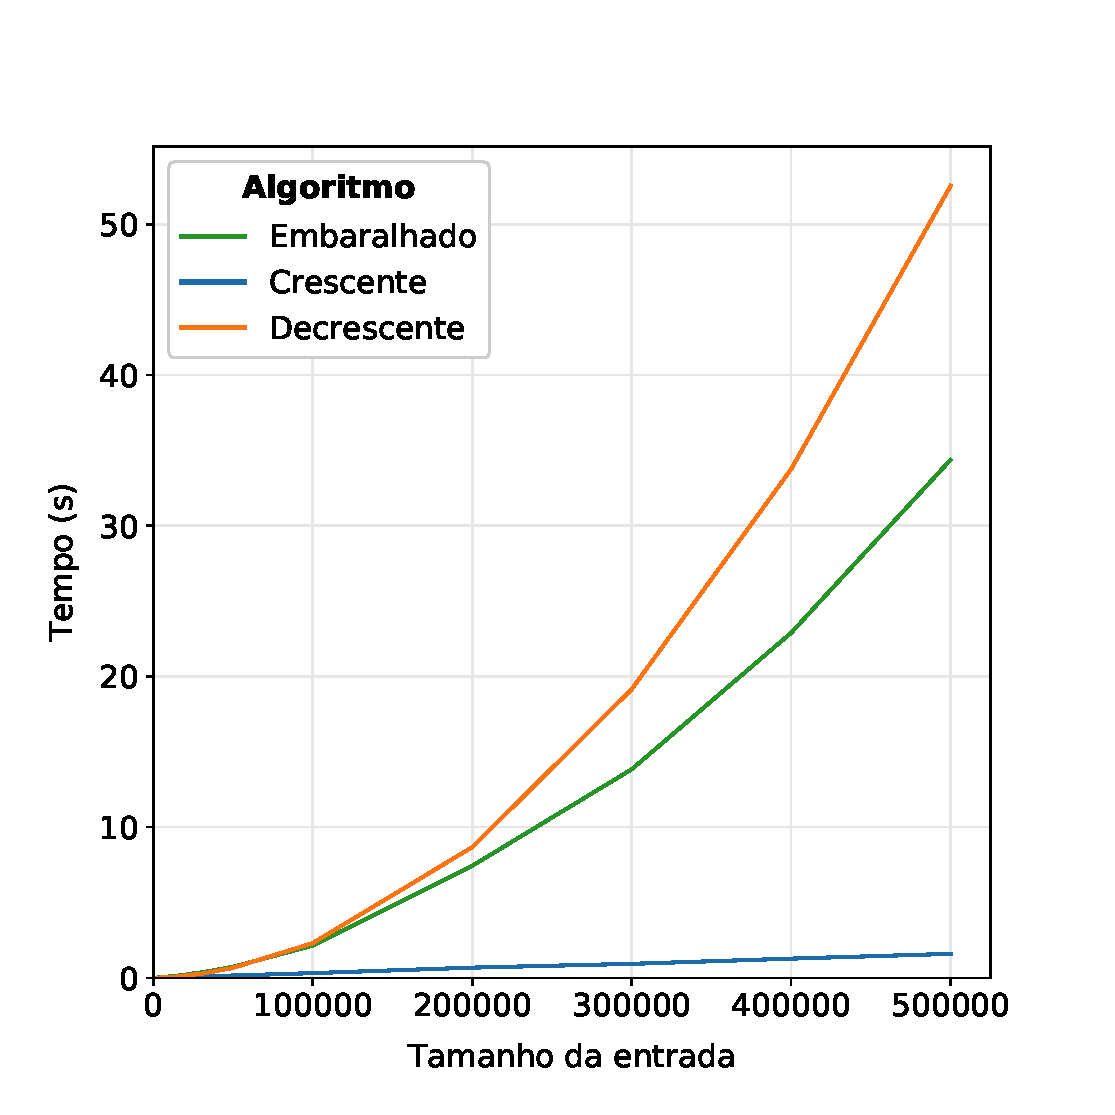
\includegraphics[width=0.5\textwidth]{shell} } \label{fig:shell_sort}
    \caption{Tempo de execução para o \textit{Shell Sort}}%
\end{figure}







\section{\textit{Heap sort}}

O \texitit{Heap sort} recebe este nome por utilizar uma \textit{heap} como estrutura de dados auxiliar para realizar a ordenação dos dados. Apesar disso, a construção da fila de prioridades ocorre sobre o conjunto de entrada, fazendo com que o algoritmo, assim como os demais apresentados até então, faça uso de memória auxiliar na ordem de $\mathcal{O}(1)$.

Este método de ordenação é descrito em alto nível por meio do Algoritmo \ref{alg:heapsort_hl}. Na primeira etapa, o conjunto de entrada é transformado em um \textit{heap} máximo, ou seja, a primeira posição do arranjo possui seu maior valor.

O objetivo da segunda etapa consiste em incrementalmente formar uma partição de elementos ordenados no fim do conjunto de entrada. Para isso, o maior elemento atual (cabeça da fila de prioridades) troca de posição com o último elemento da fila, perdendo esta posição.

Como consequência da troca, a propriedade de \textit{heap} máximo provavelmente é violada. A fim de contornar esta situação, o procedimento \texttt{update\_heap} é executado, levando em consideração agora os elementos do arranjo entre as posições $1$ e $(n-i)$, já que os elementos dali em diante formam a partição ordenada.

Cormen \cite{cormen_algorithms_ptbr} mostra que a complexidade para construção de uma \textit{heap} a partir de um \textit{array} não ordenado é da ordem de $\mathcal{O}(n)$, enquanto sua manutenção requer $\mathcal{O}(lg\,n)$ operações, etapa que é repetida $n$ vezes. Dessa forma, a complexidade do algoritmo pode ser descrita por meio da Equação \ref{eq:complex_heap}.

\begin{equation}
    \label{eq:complex_heap}
    T(n) = \Theta(n) + n\Theta(lg\,n) = max\{\Theta(n) + \Theta(nlg\,n)\} = \Theta(nlg\,n)
\end{equation}

\begin{lstlisting}[caption=Descrição do \textit{heap sort}, float, label=alg:heapsort_hl, captionpos=b]
procedure heapSort(v, n)
    v := max_heapify(v, n)      /* etapa (1) */
    
    for i:= 1 to n-1 do         /* etapa (2) */
        swap(v[1], v[n-i])
        update_heap(v, n - i)
\end{lstlisting}

Os resultados experimentais são exibidos na Figura \ref{fig:heap_sort}, onde é possível verificar que, conforme descrito pela notação $\Theta$, o \textit{heap sort} apresenta comportamento semelhante para o melhor e pior caso (conjuntos em ordem decrescente e crescente, respectivamente).

Apesar de assintoticamente mais rápido, este algoritmo é incapaz de explorar as características de entradas ordenadas (ou parcialmente ordenadas), como é o caso do \textit{Insertion sort}. Tendo em vista tal limitação, Dijkstra \cite{smoothsort} apresenta o algoritmo \textit{Smooth sort} como uma variação do \textit{Heap sort}, capaz de processar um conjunto de entrada ordenada em $\mathcal{O}(n)$ operações.

\begin{figure}[!h]%    
    \subfloat[]{{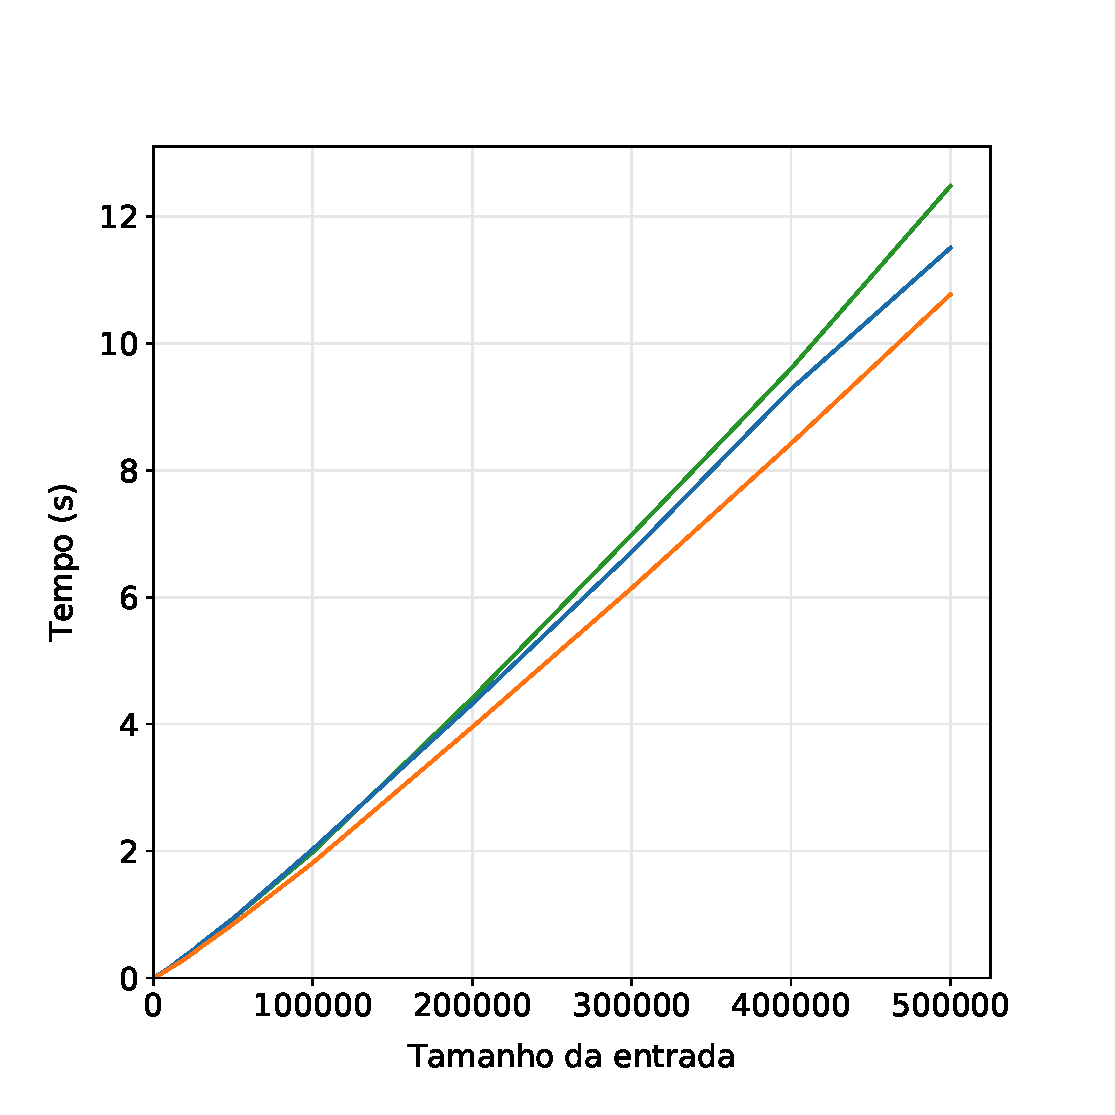
\includegraphics[width=0.5\textwidth]{heap} } \label{fig:heap_sort}}%
    \subfloat[]{{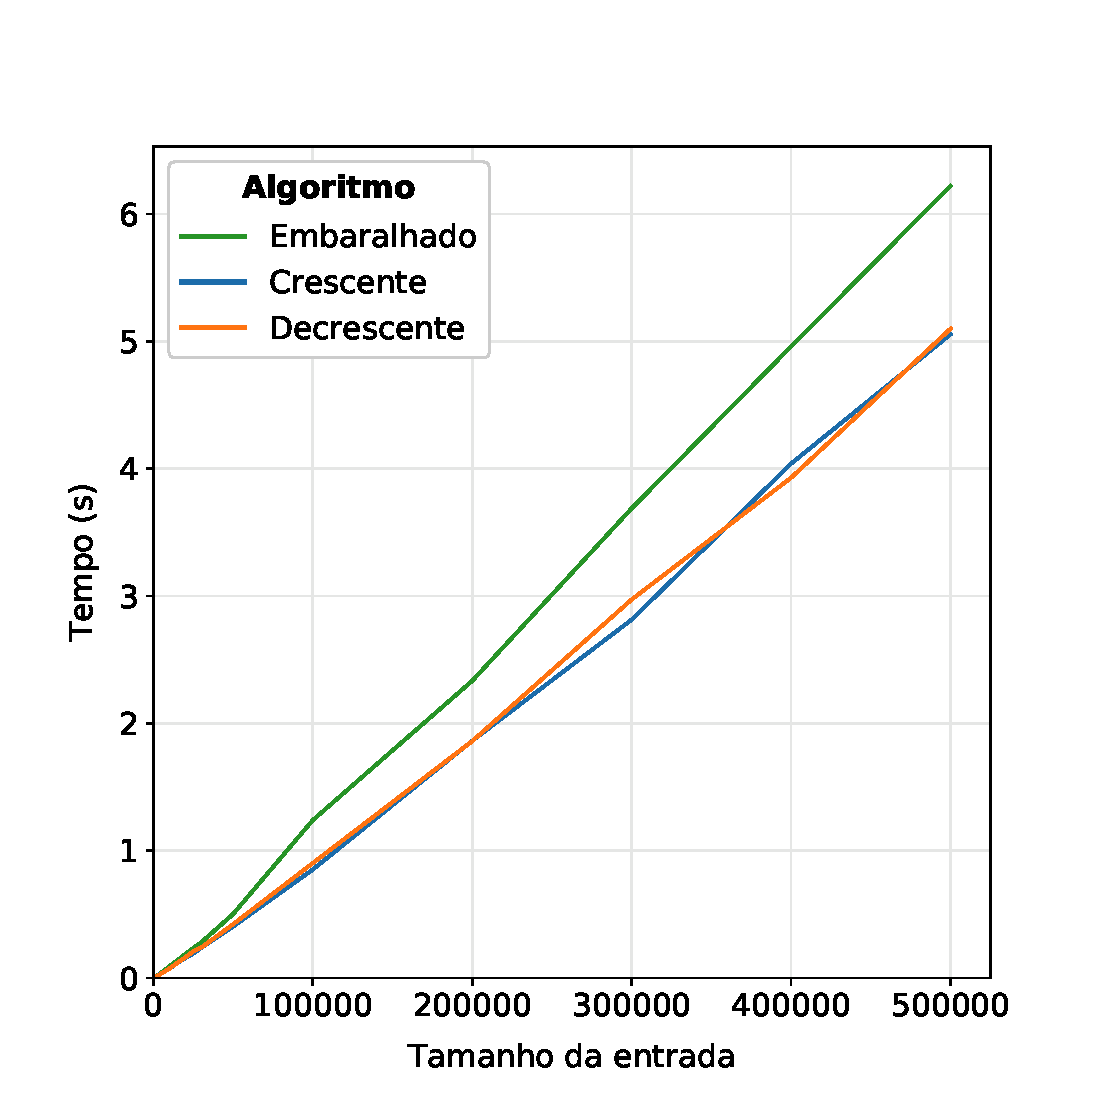
\includegraphics[width=0.5\textwidth]{merge} } \label{fig:merge_sort}}%
    \caption{Tempos de execução experimentais para o \textit{heap} (a) e \textit{merge sort} (b)}%
\end{figure}





\section{Merge sort}

O \textit{Merge sort} consiste em um algoritmo de divisão e conquista. Logo, sua análise é realizada por meio de suas fases de divisão, conquista e combinação.

O primeiro passo do algoritmo consiste em dividir o conjunto de entrada em dois sub-arranjos de tamanhos iguais, que são encaminhados para a fase de conquista. Neste momento, se o sub-arranjo em questão possuir tamanho 1, o mesmo é considerado em ordem, caso contrário este é ordenado por meio da aplicação recursiva do \textit{Merge sort}.

Por fim, a fase de combinação consiste em intercalar os sub-arranjos ordenados, a fim de obter a solução ordenada para o sub-problema. O Algoritmo \ref{alg:merge_sort} apresenta esta ideia.

\begin{lstlisting}[caption=\textit{Merge sort}. A notação \texttt{v[a:b]} representa a criação de um novo arranjo contendo os elementos de \texttt{v} no intervalo \texttt{[a,b]}. A divisão inteira é representada por \texttt{x//y}, float, label=alg:merge_sort, captionpos=b, h]
procedure mergeSort(v, start, end)
    if (end - start <= 1)
        return v
        
    /* 1. divisao */
    middle := n // 2
    left := v[start:middle]
    right := v[middle+1:end]
    
    /* 2. conquista */
    left  := mergeSort(left, start, middle)
    right := mergeSort(right, middle+1, end)
    
    /* 3. combinacao */
    return merge(left, right)
\end{lstlisting}

A etapa de divisão realiza $\Theta(n)$ operações, já que além de determinar o ponto médio do conjunto de entrada, esta também copia os elementos do arranjo original em \texttt{left} e \texttt{right}. A seguir, cada metade é ordenada recursivamente com custo $T(n/2)$, totalizando $2T(n/2)$ operações. Finalmente, os sub-arranjos ordenados são intercalados em \texttt{merge}, que simplesmente percorre os elementos de \texttt{left} e \texttt{right} inserindo-os ordenadamente, com custo $\Theta(n)$. 

Com base nesta análise é possível expressar o algoritmo por meio da Equação \ref{eq:complex_merge_quick}, que consiste no segundo caso do Teorema Mestre, reduzindo sua complexidade a $\Theta(n lg\,n)$.

\begin{equation}
    \label{eq:complex_merge_quick}
    T(n) = 2T(n/2) + \Theta(n)
\end{equation}

É importante notar que apesar de eficiente em termos de tempo, este algoritmo possui complexidade $\mathcal{O}(n)$ em termos de espaço, já que o conjunto de entrada deve ser copiado para então ser intercalado.

Os resultados experimentais obtidos são apresentados na Figura \ref{fig:Merge_sort}. Diferentemente de todos outros algoritmos apresentados, o pior caso de execução do \textit{Merge sort} consiste no conjunto de entrada não ordenado. Já entradas em ordem crescente e decrescente apresentam tempos de execução bastante próximos.

Uma possível justificativa para este comportamento se deve a forma como a intercalação ocorre. Para ambas configurações ordenadas, esta etapa consiste em copiar todos os elementos de \texttt{left} e então \texttt{right} para o arranjo destino (ou o contrário para entradas em ordem decrescente). Já para entradas embaralhadas, ora elementos de \texttt{left}, ora de \texttt{right} são copiados, o que faz com que o algoritmo cause \textit{cache misses}.

Outra possível justificativa seria o fato das \textit{branch predictions} que benificiam o algoritmo para as entradas ordenadas falharem quando o conjunto de entrada está embaralhado.






\section{Quick sort}

A estratégia deste algoritmo também se baseia na abordagem de divisão e conquista. Neste caso, a etapa de divisão particiona o arranjo em dois segmentos, $v[1..q-1]$ e $v[q+1..n]$, de forma que os elementos da primeira região sejam menores que o valor $v[q]$, chamado pivô, enquanto os elementos da sejam maiores que $v[q]$.

Assim como no \textit{Merge Sort}, a etapa de conquista consiste em ordenar ambas partições do arranjo aplicando recursivamente o algoritmo \textit{Quick Sort}. Como neste caso a ordenação ocorre sobre o \textit{array}, não há a necessidade de unir as partições na fase de combinação. Consequentemente, o uso de memória deste algoritmo, diferentemente do anterior, é $\mathcal{O}(1)$. Seu funcionamento geral é descrito no Algoritmo \ref{alg:quick_sort}, onde o funcionamento de \texttt{splitInput} é omitido.

\begin{lstlisting}[caption=\textit{Quick sort}, float, label=alg:quick_sort, captionpos=b, h]
procedure quickSort(v, start, end)
    if (end - start > 1)
        q = splitInput(v, start, end)
        quickSort(v, start, q-1)
        quickSort(v, q+1, end)
\end{lstlisting}

A etapa de divisão (particionamento) possui complexidade $\Theta(n)$, já que após a determinação do pivô, as partições devem ser formadas. Idealmente, $q$ deve ser escolhido de modo que ambos segmentos possuam o mesmo tamanho, fazendo com que o trabalho de ordenação seja dividido igualmente entre as duas chamadas recursivas do algoritmo. Essa característica também faz com que o método seja descrito pela Equação \ref{eq:complex_merge_quick}.

Apesar disso, $q$ pode ser escolhido de forma que $v[q]$ seja o menor (ou maior) elemento do arranjo atual. Como consequência, uma partição ficará vazia, ao passo que a outra irá conter os demais $n-1$ elementos do \textit{array}. Se essa situação se repetir em todos os níveis de recursão, o algoritmo apresentará o comportamento descrito pela Equação \ref{eq:quick_worst_case}, que por sua vez é de ordem quadrática.

\begin{equation}
    \begin{aligned}
        T(n) = &\; T(n-1) + \Theta(n) \\
             = &\; n\Theta(n) = \Theta(n^2)
    \end{aligned}
    \label{eq:quick_worst_case}
\end{equation}

Esta situação ocorre, por exemplo, quando o conjunto de entrada já está em ordem, seja crescente ou decrescente, e o pivô é sempre escolhido como o primeiro, ou o último, elemento da partição a ser ordenada, cenário que pode ser revertido escolhendo o elemento central da partição como pivô.

Apesar disso o problema não é removido, apenas configuração do conjunto de entrada deve ser alterada para que o algoritmo seja novamente degenerado para o caso quadrático. É possível afirmar, então, que a escolha do pivô é bastante importante, já que o mesmo tem influência direta sobre o comportamento assintótico do algoritmo.

Sedgewick \cite{algorithms_redbook} apresenta o uso de uma estratégia de amostragem a fim de aproximar o pivô da mediana real da partição sendo ordenada, aumentando as chances de uma divisão ideal. Cormen \cite{cormen_algorithms_ptbr} analisa o comportamento do \textit{Quick sort} e mostra que mesmo para divisões desbalanceadas constantes o algoritmo ainda é $\mathcal{O}(nlg\,n)$.

Além de controlar o tamanho das partições e influenciar o comportamento assintótico do algoritmo, a escolha do pivô também determina a quantidade de chamadas recursivas realizadas pelo mesmo. No caso ideal (onde os arranjos são sempre divididos ao meio) $lg(n)$ recursões ocorrem e a mesma quantidade de \textit{stack frames} é criada. Já no pior caso, o programa em execução necessitará criar $\mathcal{O}(n^2)$ \textit{frames} para ordenar o conjunto de entrada, podendo causar estouro de pilha, dependendo do tamanho do arranjo em questão.

Uma forma de contornar este problema consiste em implementar a versão iterativa do algoritmo, armazenando as posições de divisão dos sub-arranjos em uma pilha. Entretanto isso faz com que a complexidade do algoritmo, em termos de espaço, deixe de ser constante e se torne $\mathcal{O}(lg\,n)$ no caso médio e $\mathcal{O}(n^2)$ no pior caso.

Essa situação foi comprovada experimentalmente, onde a implementação recursiva do algoritmo passou a causar estouro de pilha em entradas ordenadas com mais de 500 elementos. Note que o tamanho deste conjunto de dados é inferior a menor entrada utilizada nos outros experimentos.

A fim de comparar este algoritmo de ordenação com os demais, sua versão iterativa foi utilizada. A Figura \ref{fig:quick_rec_itr_plot} mostra que o tempo de execução para as duas versões do \textit{Quick sort} é praticamente a mesma para o caso médio.

Os resultados práticos para a ordenação de outros arranjos são apresentados na Figura \ref{fig:iquick}, onde é possível observar que, além de  apresentar comportamento semelhante para entradas em ordem crescente e decrescente, conforme previsto pela análise teórica, seus tempos de execução são significativamente maiores quando comparados à ordenação de entradas embaralhadas.

A seguir, o algoritmo iterativo é modificado de modo que o elemento central, ao invés do primeiro valor da partição sendo ordenada, seja utilizado como pivô. Esta alteração reduz drasticamente o tempo de execução para as entradas ordenadas, conforme mostra a Figura \ref{fig:iquick_median}. Observe que o tamanho dos conjuntos de entrada neste gráfico são significativamente maiores que os utilizados na versão inicial do \textit{Quick sort} iterativo.

\begin{figure}[H]%
    \subfloat[]{{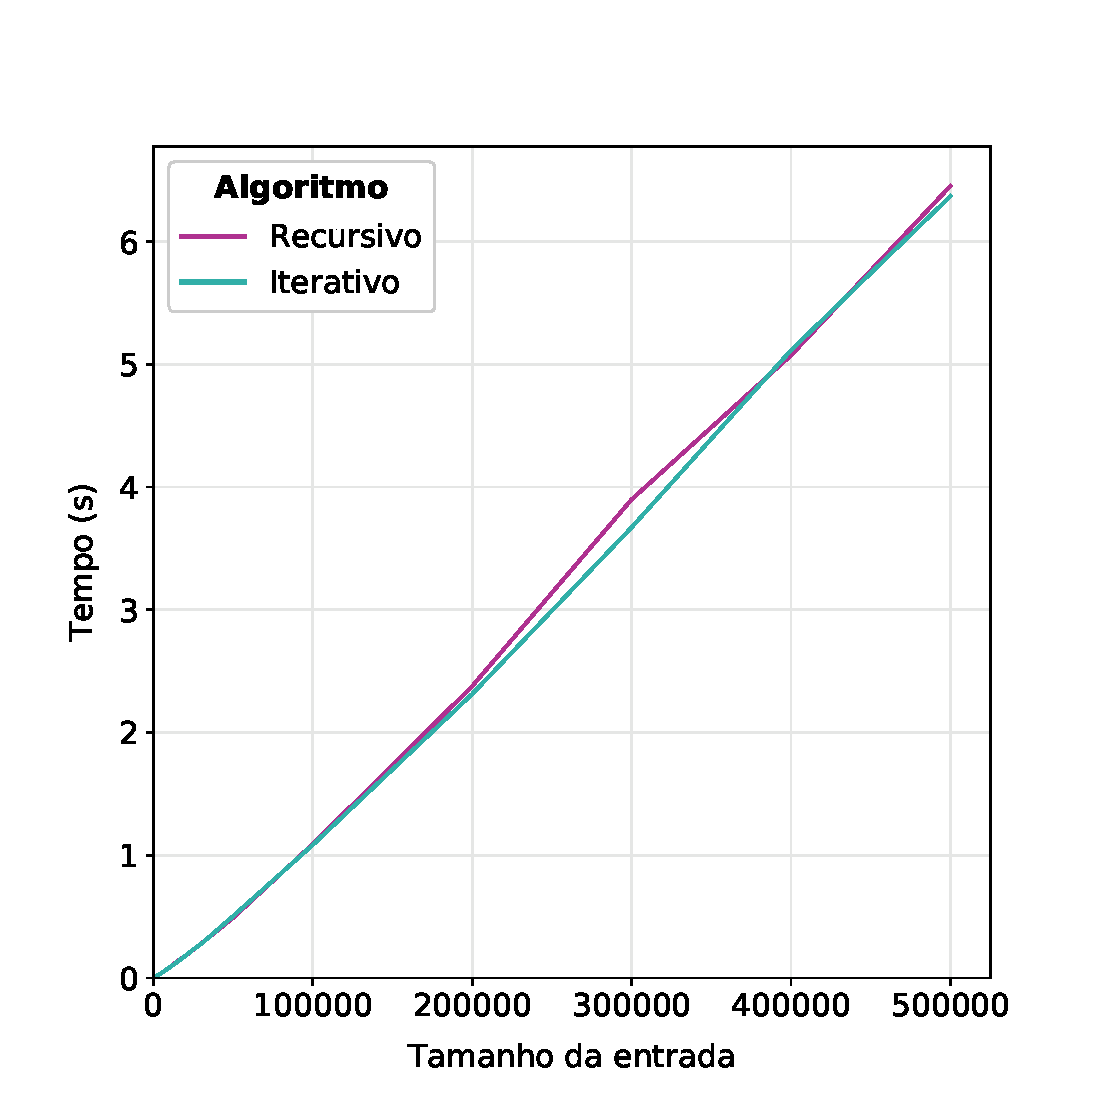
\includegraphics[width=0.5\textwidth]{quick_iquick} } \label{fig:quick_rec_itr_plot}}%
    \subfloat[]{{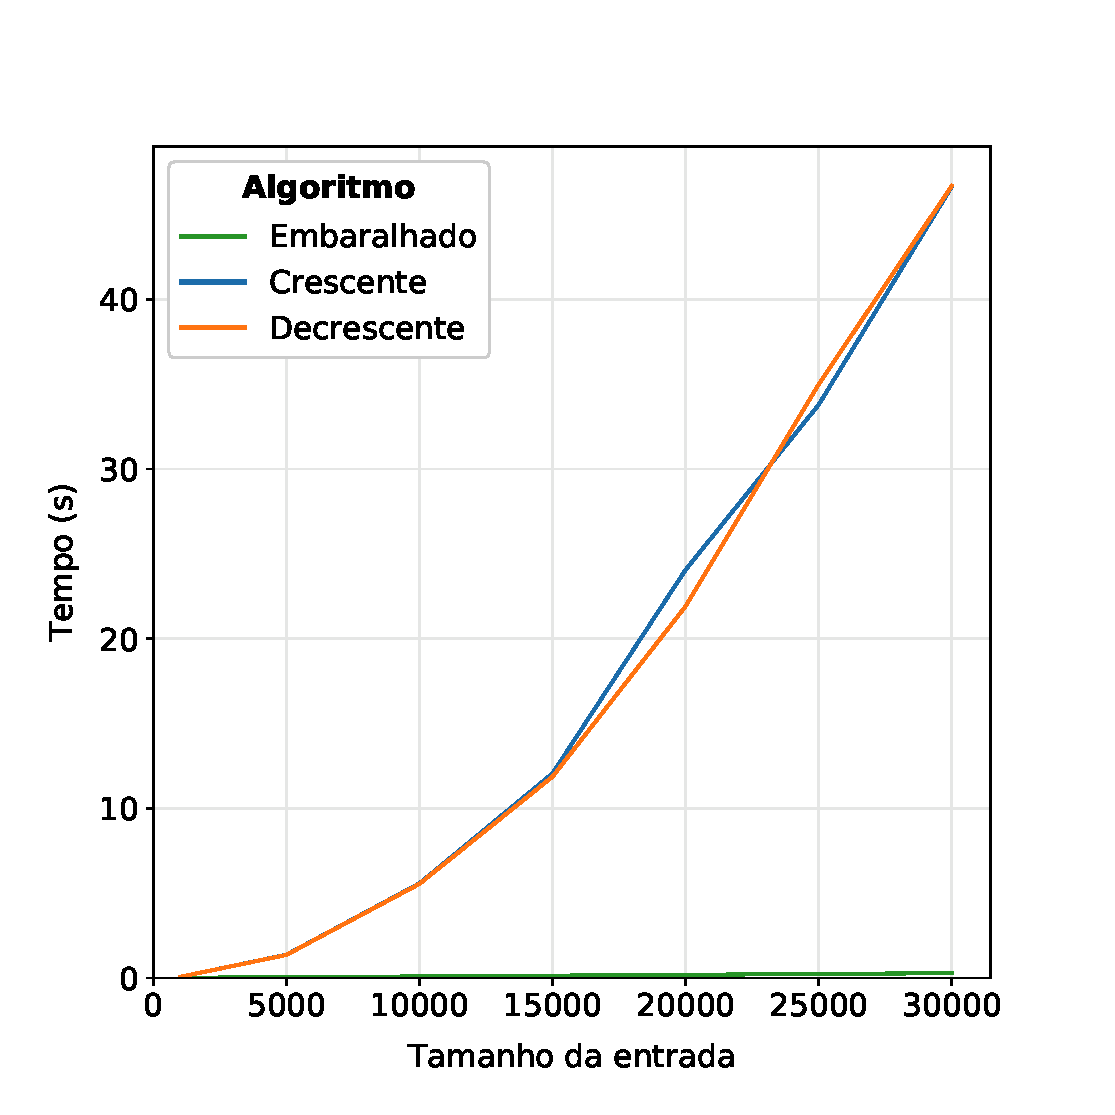
\includegraphics[width=0.5\textwidth]{iquick} } \label{fig:iquick}}%
    
    \subfloat[]{{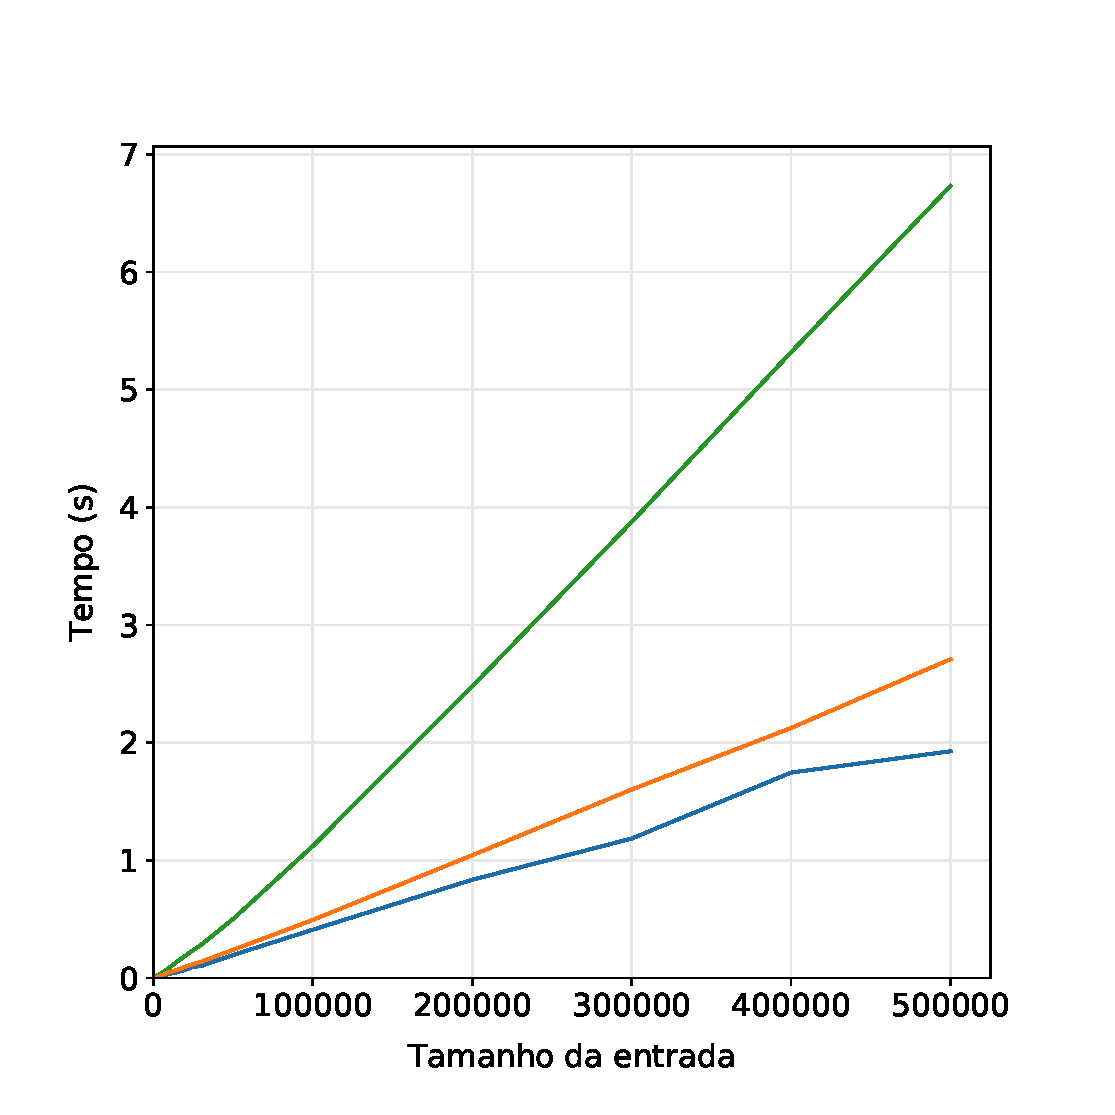
\includegraphics[width=0.5\textwidth]{iquick_median} } \label{fig:iquick_median}}%
    \subfloat[]{{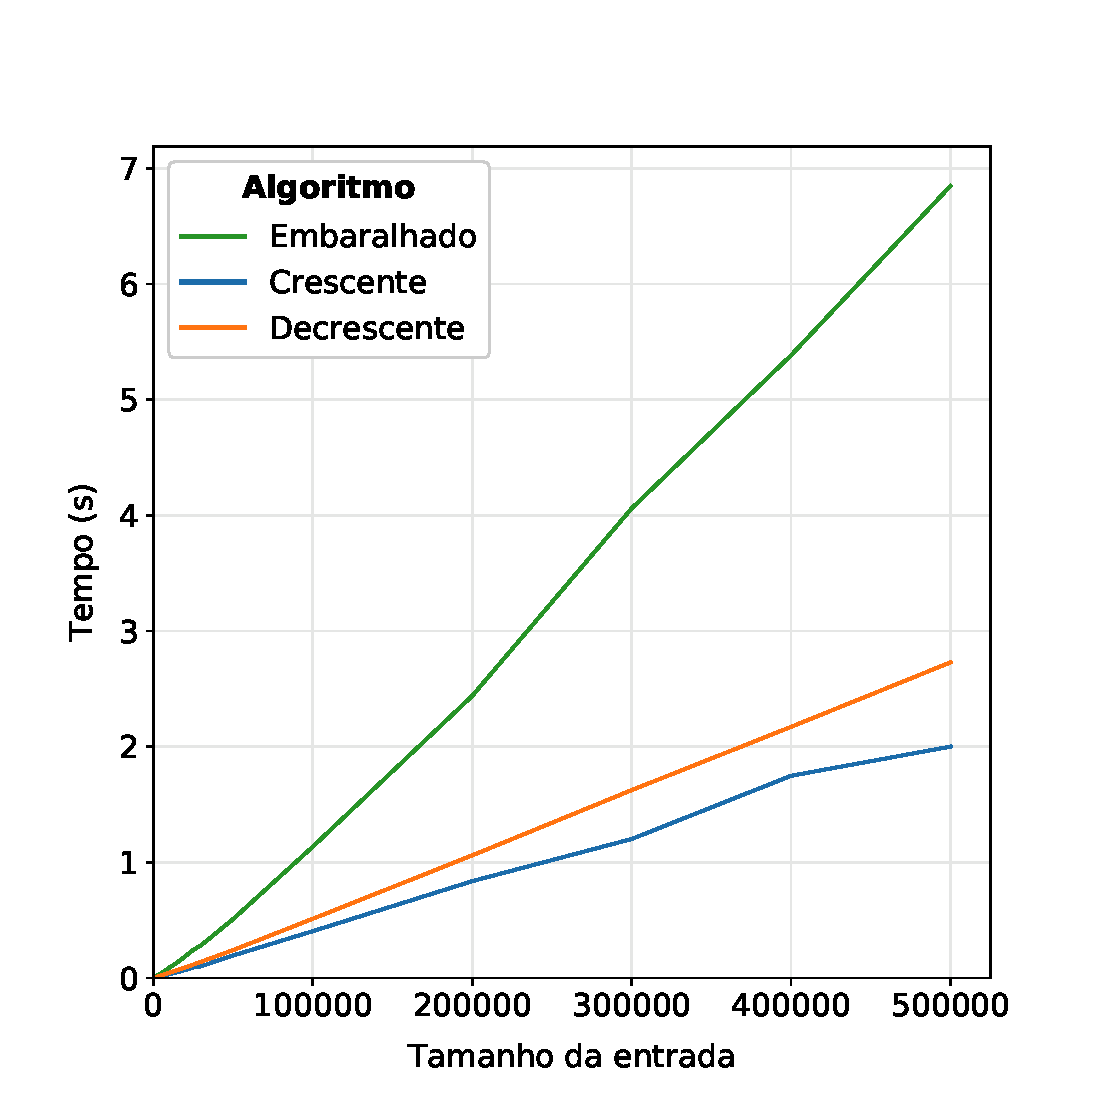
\includegraphics[width=0.5\textwidth]{quick_median} } \label{fig:quick_median}}%
    
    \caption{Variações na implementação do \textit{Quick Sort}. (a) tempos de execução entre as implementações recursiva e iterativa. (b) comportamento do algoritmo iterativo para diferentes entradas. (c) implementação iterativa utilizando o elemento central do arranjo como pivô. (d) comportamento do algoritmo recursivo utilizando o elemento central como pivô.}%
\end{figure}

Enquanto a implementação que utiliza o primeiro elemento da partição requer 46.69 segundos para ordenar um conjunto de 30 mil elementos, o mesmo algoritmo, utilizando o elemento central da partição como pivô, requer apenas 0.28 segundos para realizar a mesma operação. Além disso, ao realizar esta alteração, apesar de todos conjuntos de teste  utilizadas agora se enquadrarem no caso médio, as entradas ordenadas tornam-se o melhor caso prático. Isso ocorre pois a divisão dos sub-arranjos em seus elementos centrais geram partições de tamanhos idênticos, consistindo no caso ideal. Esta mesma situação não ocorre na entrada embaralhada, onde nem sempre a divisão de partições ocorre de maneira balanceada.

Novamente, a alteração não resolve o problema da complexidade quadrática do algoritmo, já que ainda é possível construir um conjunto de entrada que faça com que o tempo de execução do algoritmo seja degenerado para o pior caso. Um método capaz de gerar tais conjuntos de entrada é apresentado em \cite{quicksort_killer}.

Por fim, a Figura \ref{fig:quick_median} mostra que a alteração na estratégia de escolha do pivô também evita o estouro de pilha, corroborando com a hipótese que esta escolha também influencia no nível de profundidade da pilha de recursão.

É possível perceber que estes resultados são extremamente similares àqueles obtidos utilizando a versão iterativa do algoritmo com pivô central. Na realidade, conforme dito anteriormente, estes métodos diferem apenas em termos de sua complexidade de espaço.

Apesar de todas estas considerações, o \textit{Quick Sort} apresenta baixo tempo de execução devido a sua pequena constante oculta. Além disso, o algoritmo pode ser implementado em poucas linhas de código, tornando-o competitivo com outros métodos. Finalmente, boas estratégias para escolha de pivô podem ser utilizadas a fim de diminuir a probabilidade do algoritmo vir a se comportar de maneira quadrática.

Outra forma de contornar este problema é a utilização de um algoritmo híbrido, como é o caso do \textit{Introspective Sort} (ou \textit{introsort}), método procede como o \textit{Quick sort}, mas passa a funcionar como o \textit{Heap sort} tão logo um determinado limite no nível de recursão é atingido.
    
\section{Comparações Gerais}

A Figura \ref{fig:all_sorts} relaciona o desempenho de todos algoritmos apresentados até então. Para o \textit{Quick sort} apenas sua implementação iterativa foi utilizada, já que esta é equivalente à recursiva, em termos de tempo de execução.

No gráfico os algoritmos dividem-se dois conglomerados, à esquerda encontram-se aqueles de complexidade quadrática, mostrando-se extremamente custosos quando comparados aos da direita, com complexidade $\mathcal{O}(nlg\,n)$ e $\mathcal{O}(n^{\nicefrac{3}{2}})$. Esta figura também reforça a justifica de utilizar arranjos com até 30 mil elementos para a análise dos métodos de ordenação quadráticos.

Por meio do gráfico da Figura \ref{fig:quadratics} é possível concluir que o \textit{Selection sort} é o algoritmo mais rápido de ordem quadrática. Apesar disso, deve-se considerar as possíveis utilizações práticas dos demais.

O \textit{Bubble sort} apesar de ser o método mais lento, assim como sua versão melhorada, é implementado facilmente, tornando-o interessante para a prototipação, quando não se tem acesso rápido a outras formas de ordenar um arranjo.

O \textit{Insertion sort} é linear para entradas ordenadas e poder ser melhorado na forma \textit{Shell sort}. Apesar disso, este é o único algoritmo apresentado capaz de realizar ordenações \textit{online}, ou seja, adicionar valores não observados anteriormente na partição ordenada de maneira eficiente.

\begin{figure}[H]%
    \centering
    \subfloat[]{{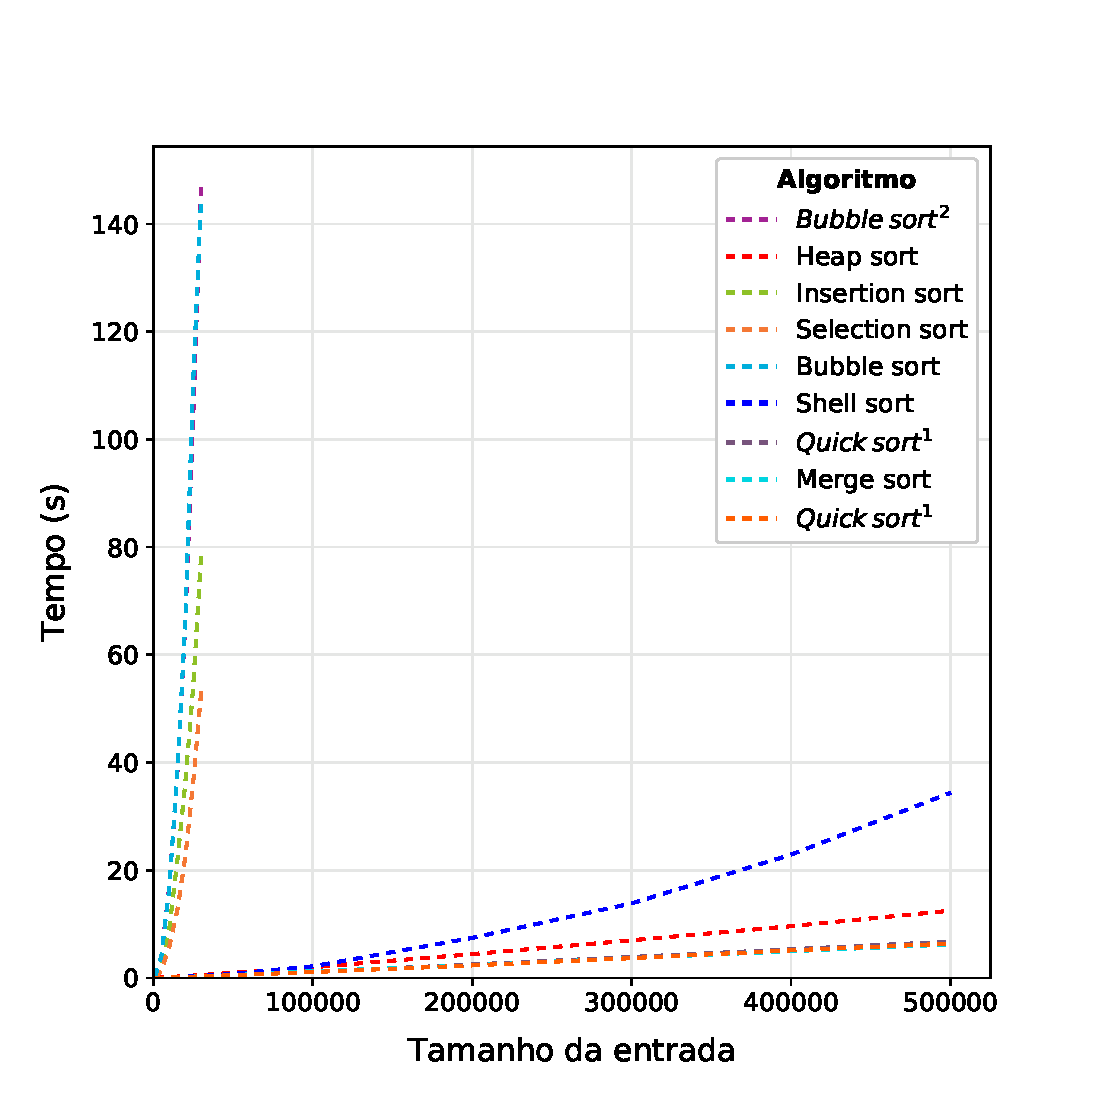
\includegraphics[width=0.7\textwidth]{all} } \label{fig:all_sorts}}%
    
    \subfloat[]{{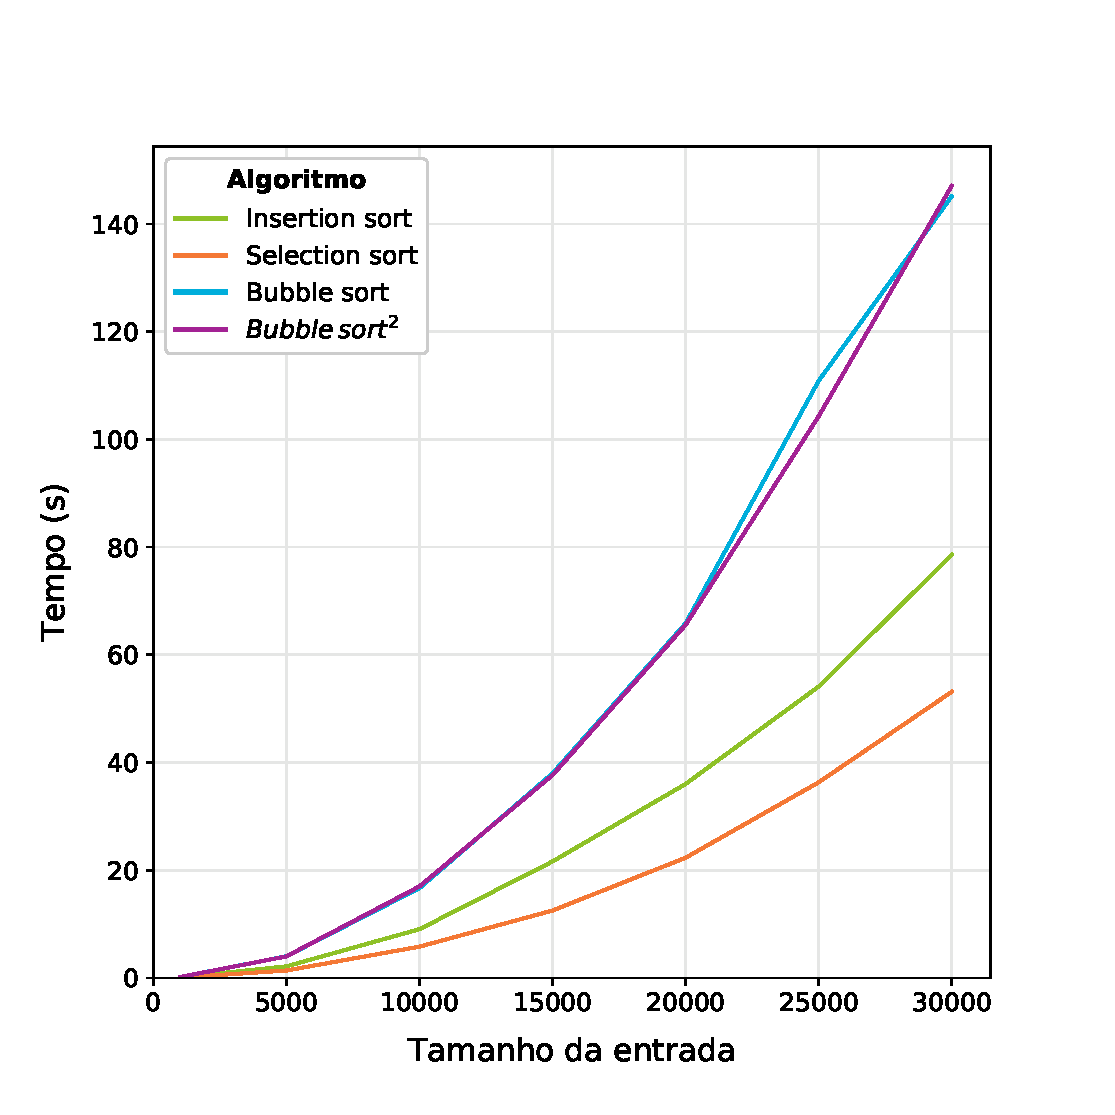
\includegraphics[width=0.5\textwidth]{quadratics} } \label{fig:quadratics}}%
    \subfloat[]{{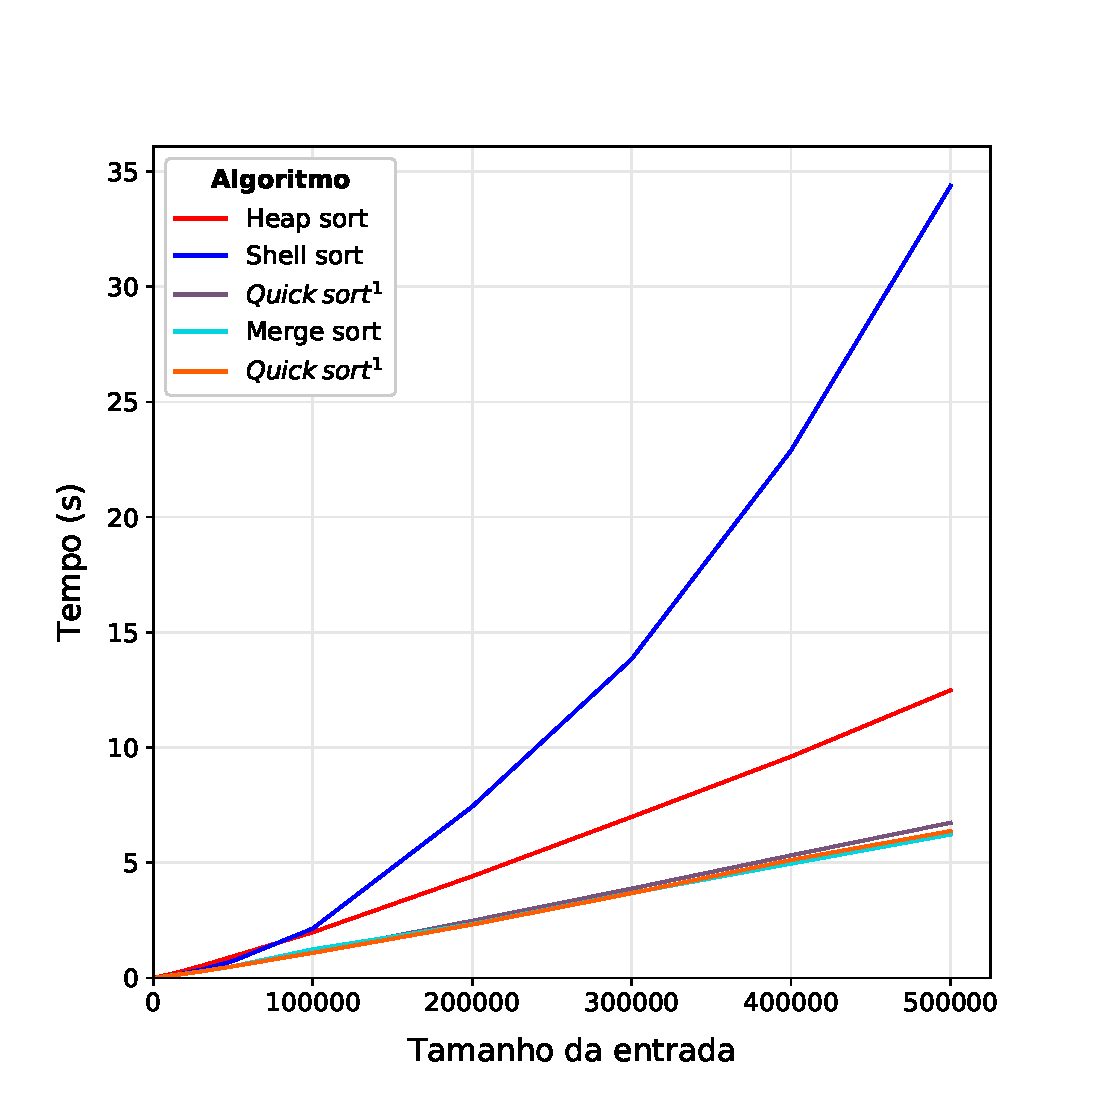
\includegraphics[width=0.5\textwidth]{log_linear} } \label{fig:log_linear}}%

    \caption{Comparação do tempo de execução entre todos algoritmos analisados em seu caso médio. $^1$indica implementação iterativa. $^2$é a implementação melhorada do \textit{Bubble sort}}%
\end{figure}

Já da Figura \ref{fig:log_linear} mostra que os algoritmos \textit{Quick} e \textit{Merge sort} são os mais rápidos, com desempenhos praticamente iguais. Apesar disso, o último método requer $\Theta(n)$ posições de memória para realizar a ordenação, enquanto que o primeiro utiliza $\mathcal{O}(1)$ se uma boa estratégia para a escolha do pivô for utilizada, consequentemente diminuindo as chances de ocorrência do seu pior caso de execução. Entretanto, uma vantagem do \textit{Merge} sobre o \textit{Quick sort} é o fato deste ser estável, ou seja, elementos iguais não têm sua precedência alterada durante processo de ordenação.

O \textit{Shell sort} pode ser visto como uma melhoria que pode ser implementada rapidamente sobre o \textit{Insertion sort}, preservando seu bom desempenho para entradas parcialmente ordenadas. Apesar de mais lento que os demais métodos, a ordenação ocorre no lugar (diferentemente do \textit{Merge sort}) e não há a necessidade de determinar o pivô para ordenação, fator que pode dificultar a implementação rápida do \textit{Quick sort}.

O \textit{Heap sort} é uma escolha intermediária entre os algoritmos mais eficientes, em termos de tempo computacional e também não utiliza memória auxiliar. Apesar disso, sua implementação é mais extensa e suscetível a erros.

\section{Conclusão}

Neste trabalho foram comparados os tempos de execução entre diferentes algoritmos de ordenação e suas respectivas complexidades assintóticas. É possível concluir que os resultados teóricos apresentam uma boa base para comparar os algoritmos e condizem com os resultados práticos.

Já a análise prática evidencia particularidades dos algoritmos para entradas com diferentes configurações, além de permitir sua comparação direta no mesmo ambiente de testes. Fatores práticos, impossíveis de serem considerados no primeiro tipo de análise também são considerados, como é o caso do aproveitamento das linhas de \textit{cache} e \textit{branch predictions} realizadas pelo processador. Naturalmente, os resultados aqui obtidos estão limitados à configuração de \textit{hardware} e \textit{software} utilizada, impossibilitando comparar algoritmos distintos testados em ambientes diferentes.

Finalmente, em termos de escolha de algoritmos, \textit{Quick} e \textit{Merge sort} são preferíveis quando se deseja ordenação rápida e espera-se que o conjunto de entrada esteja embaralhado na maioria dos casos. Apesar disso, a utilização de algoritmos que apresentam desempenho pior que estes no caso médio podem levar a resultados melhores em situações específicas.

\printbibliography

\end{document}
